\documentclass[numbers]{assets/matterlab}
% Packages used by the MAPPA preprint; the class supplies layout and fonts.
\usepackage{amsmath,amssymb,mathtools}
\usepackage{xurl}
\usepackage{float}
\usepackage{algorithmic}
\floatstyle{ruled}
\newfloat{algorithm}{tbp}{loa}
\floatname{algorithm}{Algorithm}
\floatstyle{plain}
\usepackage[noabbrev,nameinlink]{cleveref}
\hypersetup{pdftitle={MAPPA: Symmetry-Aware Atom Mapping through Continuous Fragment Growth},pdfauthor={Yunheng Zou and coauthors}}
\setcounter{topnumber}{3}
\renewcommand{\topfraction}{0.9}
\renewcommand{\textfraction}{0.08}
\renewcommand{\floatpagefraction}{0.7}

% Avoid isolated first/last lines at page boundaries.
\clubpenalty=10000
\widowpenalty=10000

% Generated from separately scoped current and historical evidence.
\newcommand{\CurrentGoldenRecovered}{1,830}
\newcommand{\CurrentGoldenTotal}{1,851}
\newcommand{\CurrentGoldenPercent}{98.87}
\newcommand{\CurrentGoldenDirections}{3,702}
\newcommand{\CurrentGoldenDirectionRecovered}{3,618}
\newcommand{\GoldenOneRecovered}{1,834}
\newcommand{\GoldenOnePercent}{99.08}
\newcommand{\GoldenThreeRecovered}{1,837}
\newcommand{\GoldenThreePercent}{99.24}
\newcommand{\GoldenTenRecovered}{1,840}
\newcommand{\GoldenTenPercent}{99.41}
\newcommand{\GoldenTenUnknown}{0}
\newcommand{\SlapRecovered}{1,796}
\newcommand{\SlapPercent}{97.03}
\newcommand{\RecoveryDifference}{2.05}
\newcommand{\CommonCases}{1,821}
\newcommand{\OneCPU}{2.52}
\newcommand{\TwoCPU}{4.95}
\newcommand{\SlapCPU}{4.82}
\newcommand{\AamOnly}{43}
\newcommand{\SlapOnly}{5}
\newcommand{\SweepRecovered}{162}
\newcommand{\SweepClasses}{168}
\newcommand{\SlapAbsent}{52}
\newcommand{\SlapUnknown}{3}
\newcommand{\FlatFamilies}{120,052}
\newcommand{\DecodedClasses}{300}

\renewcommand{\arraystretch}{1.2}
\setlength{\emergencystretch}{2em}
\title{MAPPA: Symmetry-Aware Atom Mapping through Continuous Fragment Growth}
\author[2,6,8]{Yunheng Zou}
\author[10]{Olalla Nieto Faza}
\author[11]{Shifa Hussain}
\author[2,5,\dagger]{Varinia Bernales}
\author[1,2,3,4,5,6,7,8,9,\dagger]{Al\'an Aspuru-Guzik}
% Numbering and addresses follow the affiliation reference supplied by the author.
% Olalla's university was supplied by the author; her department is confirmed
% by the university directory. Shifa's department name follows the official UTM site.
\affiliation[1]{Department of Chemistry, University of Toronto, 80 St. George St., Toronto, ON M5S 3H6, Canada}
\affiliation[2]{Department of Computer Science, University of Toronto, 40 St George St., Toronto, ON M5S 2E4, Canada}
\affiliation[3]{Department of Materials Science \& Engineering, University of Toronto, 184 College St., Toronto, ON M5S 3E4, Canada}
\affiliation[4]{Department of Chemical Engineering \& Applied Chemistry, University of Toronto, 200 College St., Toronto, ON M5S 3E5, Canada}
\affiliation[5]{Acceleration Consortium, 700 University Ave., Toronto, ON M7A 2S4, Canada}
\affiliation[6]{Vector Institute for Artificial Intelligence, W1140-108 College St., Schwartz Reisman Innovation Campus, Toronto, ON M5G 0C6, Canada}
\affiliation[7]{Canadian Institute for Advanced Research (CIFAR), 661 University Ave., Toronto, ON M5G 1M1, Canada}
\affiliation[8]{NVIDIA, 431 King St. W \#6th, Toronto, ON M5V 1K4, Canada}
\affiliation[9]{Institute of Medical Science, 1 King's College Circle, Medical Sciences Building, Room 2374, Toronto, ON M5S 1A8, Canada}
\affiliation[10]{Department of Organic Chemistry, Universidade de Vigo, Spain}
\affiliation[11]{Department of Biology, University of Toronto Mississauga, 1867 Inner Circle Rd., Mississauga, ON L5L 1C6, Canada}
\contribution[\dagger]{Principal investigators}
\abstract{Atom mapping assigns corresponding atoms across a chemical reaction, but the same endpoints can support several assignments, and symmetry can multiply their explicit representations. We introduce MAPPA, a graph-based method that retains alternative fragment placements in compressed form. Fragment growth asks only whether one compatible assignment exists. When growth saturates, a separate operation constructs the distinct compressed placements, which condition the subsequent mapping of the remaining atoms. A cut sweep varies the growth conditions to explore alternative fragment boundaries. After final family aggregation, a separate decoder collects unique fragments, shares local bond-event calculations and composes them under the saved joint constraints. A completed validation on all \CurrentGoldenTotal{} Golden reactions recovers the annotated correspondence among the retained alternatives for \CurrentGoldenRecovered{} reactions (\CurrentGoldenPercent\%), with all matching, decoding and verification tasks completed and no unresolved verification outcomes. Recovery measures reference inclusion rather than top-ranked prediction accuracy. MAPPA provides an inspectable representation of atom correspondence and bond changes for subsequent chemical assessment.
}
\date{November 8, 2026}
\metadata[Status]{Preprint}
\begin{document}
\maketitle
\begin{figure}[H]
\centering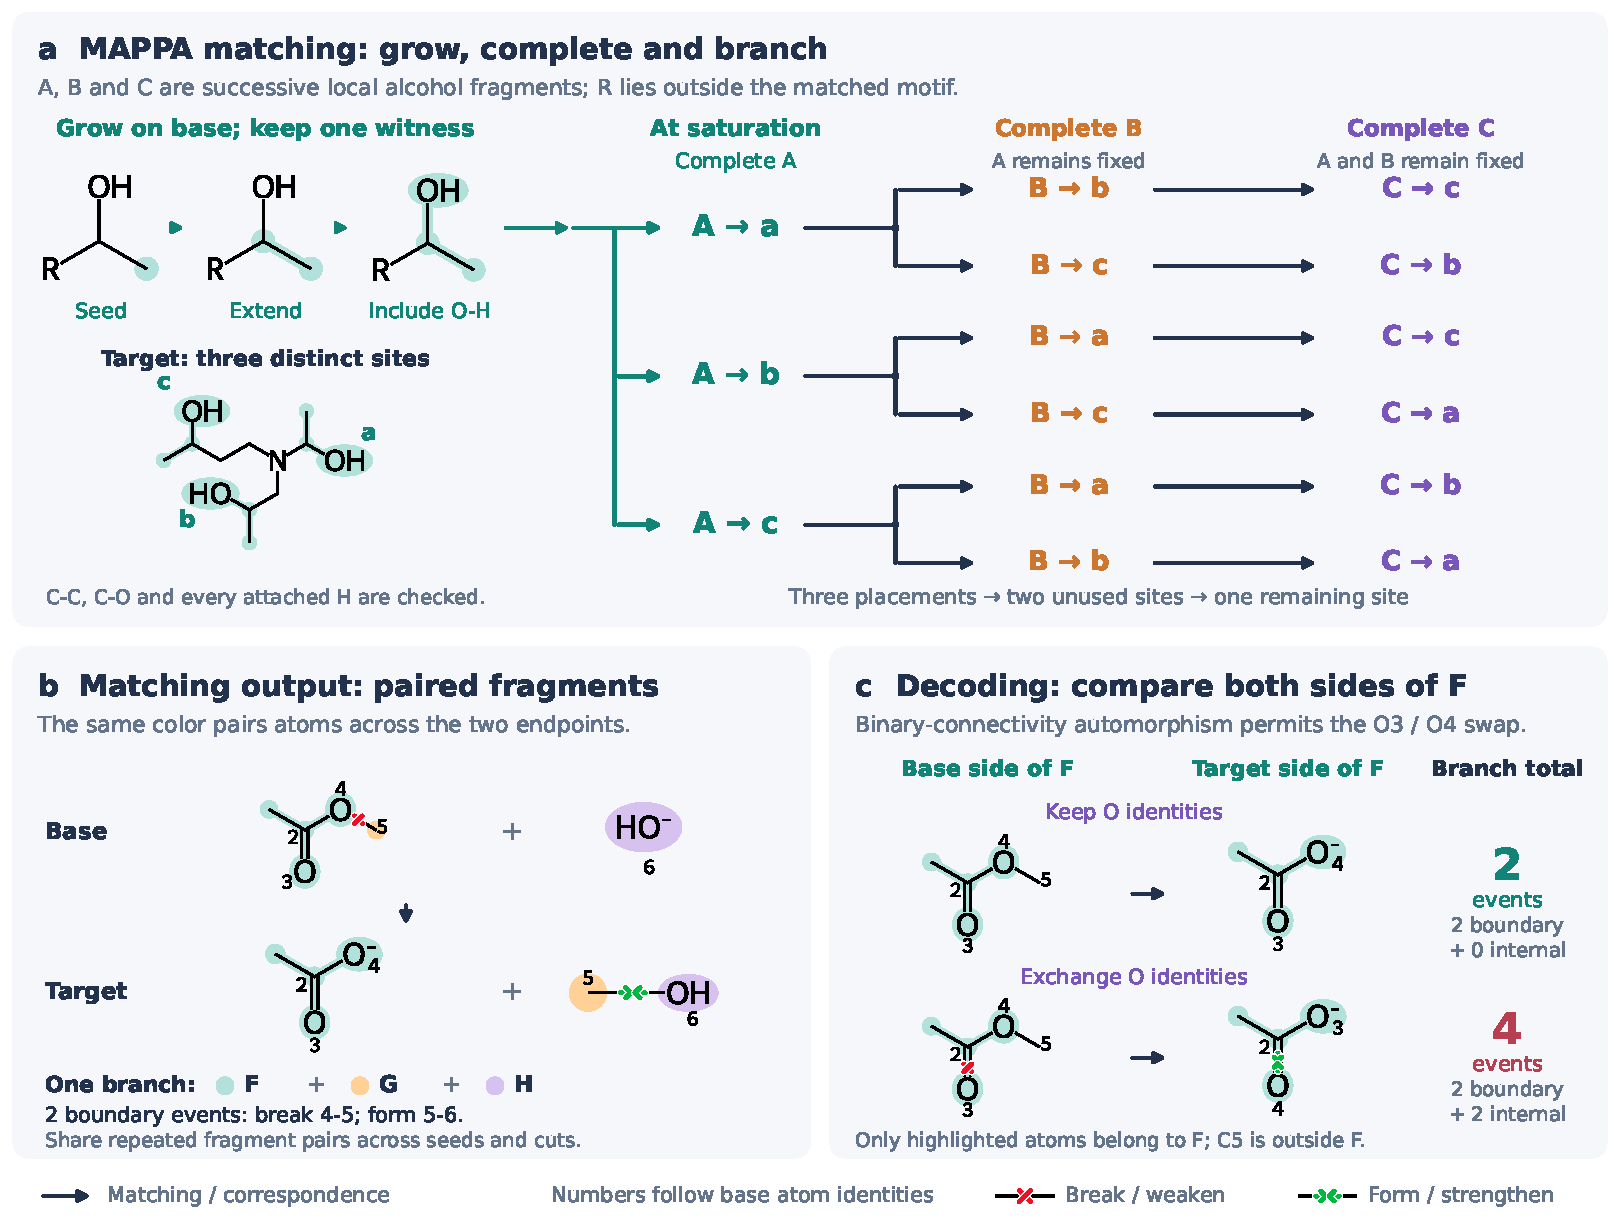
\includegraphics[width=.95\linewidth]{figs/fig1_algorithm.pdf}
\caption{\textbf{MAPPA discovers and organizes alternative atom mappings.} (a) Growth retains one witness; saturation constructs compressed placements for conditional branching. (b) Seeds and single-edge cuts contribute families to a shared catalogue. (c) Decoding reuses unique-fragment symmetry responses and combines internal, boundary and sweep-bond contributions. Red crosses mark cleavage or weakening; green arrows mark formation or strengthening. Dashed arrows project choices within a compressed family. Molecular examples and their scope are explained in \Cref{sec:algorithm-details}.}
\label{fig:algorithm}
\end{figure}
\clearpage
\input{includes/include-body}

\par\noindent\begin{minipage}{\linewidth}
\section*{Author information}
{\small\affiliationlist\par\contributionlist\par}
\begin{center}
\includegraphics[height=0.7cm]{assets/logo_matterlab.pdf}\hspace{0.5cm}
\includegraphics[height=0.7cm]{assets/nvidia-logo-vert.png}\hspace{0.5cm}
\includegraphics[height=0.7cm]{assets/logo_ac.pdf}\hspace{0.5cm}
\includegraphics[height=0.7cm]{assets/logo_uoft.pdf}\hspace{0.5cm}
\includegraphics[height=0.7cm]{assets/logo_vector.png}
\end{center}
\end{minipage}
\section*{Code and data}
Code and reproduction instructions are available at \href{https://github.com/yunhzou/MAPPA-AAM}{MAPPA source repository}, branch \texttt{main}. The repository guide \texttt{manuscript/REPRODUCIBILITY.md} links full benchmark configurations, software versions, per-case results, and figure-generation scripts. Golden and EnzymeMap are distributed by their original authors~\citep{lin2022,heid2023enzymemap}.
\par\noindent\begin{minipage}{\linewidth}
\section*{Acknowledgements}
We gratefully acknowledge the longstanding contributions of the Matter Lab’s current and past group members (matter.toronto.edu), and in particular those of the El Agente team (elagente.ca). C.C. acknowledges support from the DOE grant with the University of Minnesota, award \#A006801504, and the Basic Science Research Program through the National Research Foundation of Korea (NRF), funded by the Ministry of Education (RS-2025-02634334). Y.K. was supported by the CIFAR AI Safety Catalyst Award (Catalyst Fund Project \#CF26-AI-001). J.B.P.S. acknowledges funding of this project by the Natural Sciences and Engineering Research Council of Canada (NSERC) Alliance Grant \#ALLRP587593-23 (Quantamole). A.W. acknowledges support from the Canada Graduate Scholarships—Doctoral (CGS-D) program.

This research is part of the University of Toronto’s Acceleration Consortium, which receives funding from the CFREF-2022-00042 Canada First Research Excellence Fund. Computations were performed on the Niagara supercomputer at the SciNet HPC Consortium. SciNet is funded by the Canada Foundation for Innovation; the Government of Ontario; the Ontario Research Fund—Research Excellence; and the University of Toronto.

A.A.-G. thanks Anders G. Frøseth for his generous support and acknowledges the generous support of NSERC and the Canada 150 Research Chairs program. A.A.-G. and V.B. also acknowledge the generous support of Natural Resources Canada and the Canada 150 Research Chairs program and the University of Toronto’s Acceleration Consortium, which receives funding from the CFREF-2022-00042 Canada First Research Excellence Fund.

This work was supported by the Defense Advanced Research Projects Agency (DARPA) under Agreement No. HR0011262E022. This work was also supported by the AI2050 program of Schmidt Sciences.

Molecular graphics and analyses were performed with UCSF ChimeraX~\citep{goddard2018chimerax,pettersen2021chimerax}, developed by the Resource for Biocomputing, Visualization, and Informatics at the University of California, San Francisco, with support from National Institutes of Health R01-GM129325 and the Office of Cyber Infrastructure and Computational Biology, National Institute of Allergy and Infectious Diseases.

We thank Kjell Jorner and Robert Pollice for helpful discussions.

\par
\end{minipage}
\FloatBarrier
{\small\bibliography{references}\bibliographystyle{assets/plainnat}}
\clearpage
\appendix
\input{includes/include-appendix}
\end{document}
